%========================================================CHAPTER 1========================================================

\chapter{Introduction}\label{chap:introduction}
This paper is written for the master course \textit{Concepts of Programming Languages} of the department of computer science in the Winter Term 23/24 at the Technical University of Applied Sciences Rosenheim.
    
    \section{Background}\label{sec:background}
    According to the November 2023 TIOBE Index data, there are currently over 150 programming languages in existence. The programming landscape includes a diverse array of languages, reflecting the dynamic and ever-evolving nature of the field.\cite{Tiobeindex} When producing software, a software engineer must select a programming language that is suitable for a particular problem. This topic has been discussed for approximately 50 years.\cite{Tharp1982} The reason for this is that each language has its own paradigms and concepts. While there is no perfect language that can solve all problems, one can choose a language that fits many problems or one that is perfect for a single problem. The goal of selecting the appropriate programming language is to find one that suits the requirements and context of a given problem. This paper compares Go and F\# in the context of functional programming (FP) to cover this topic.

    \section{Purpose of the Project}\label{sec:purpose}
    The aim of this project is to analyze and compare the similarities and differences between two \ac{fp} languages: Go\footnote{Website: \url{https://go.dev} (Accessed on 12/02/2023)} and F\#\footnote{Website: \url{https://dotnet.microsoft.com/languages/fsharp} (Accessed on 12/02/2023)}. Go was chosen as the initial language due to its consistent usage throughout the course, making it a mandatory inclusion in the project. In order to conduct a comparative analysis, it is essential to include a second programming language alongside Go. For this purpose, F\# has been selected. The decision to include F\# in this study was deliberate, as explained in section\ \ref{sec:whyfsharp}. By comparing Go and F\#, this project aims to uncover the nuances and divergences in their approaches to \ac{fp} paradigms, shedding light on their distinctive features, strengths, and potential use cases. Through this comparative exploration, the project aims to provide valuable insights into the \ac{fp} landscape. It seeks to offer a nuanced understanding of the strengths and trade-offs associated with both languages.

    \section{Why F\#?}\label{sec:whyfsharp}
    One of the main reasons for selecting F\# is its status as a functional-first programming language. Unlike Go's multi-paradigm approach, F\# is committed to functional principles, providing an excellent opportunity to explore the benefits of implementing code from a pure perspective.
    For a more comprehensive understanding of F\#, including its syntax, features, and \ac{fp} principles, please refer to section\ \ref{sec:fsharp-overview} and chapter\ \ref{chap:comparison}.

    \section{Roadmap}\label{sec:roadmap}
    Chapter\ \ref{chap:project-overview} briefly discusses the \textit{NerdDeck} flashcard \ac{app} as a practical context for understanding \ac{fp} in action. Chapter\ \ref{chap:functional-programming} provides an overview of \ac{fp} principles, followed by an introduction to Go and F\# of \ac{fp} in chapter\ \ref{chap:introgoandfsharp}. Chapter\ \ref{chap:comparison} is the centerpiece of this paper, as it provides a focused exploration of two critical functional concepts: Algebraic Data Types and First-class Functions. This section uses code examples to illuminate nuances in implementation, providing a concise yet insightful comparative analysis. The paper concludes in chapter\ \ref{chap:conclusion}, summarizing challenges and outlook from both the project and the comparison. This streamlined roadmap ensures
    a comprehensive yet condensed examination of \ac{fp} in Go and F\#.


%========================================================CHAPTER 2========================================================

\chapter{Project Overview}\label{chap:project-overview}
    \section{Description of the \textit{NerdDeck} flashcard Application}\label{sec:descriptionofnerddeck}
    This coding project aims to compare and contrast the use of \ac{fp} in Go and F\#. The \textit{NerdDeck} \ac{app} is designed to aid in memorization using flashcards. A similar product, Anki\footnote{Website: \url{https://apps.ankiweb.net} (Accessed on 12/03/2023)}, already exists for this purpose, with most of its components written in Rust and Python. However, \textit{NerdDeck} stands out as it is written twice, once in Go and once in F\#, utilizing the \ac{fp} paradigm. In section\ \ref{sec:fsharp-overview}, F\# will not pose any issues since it allows for functional-first code. However, since Go is an impure language, the objective is to write in a functional manner as much as possible.\ \textit{NerdDeck} adheres to the project framework by using the \ac{cli} as a \ac{gui}, while Anki has its own developed interface.

    \section{Requirements}\label{sec:requirements}
    The \ac{app} should enable a single user to utilize the \ac{sm2} algorithm, which is employed for a learning technique known as spaced repetition.\cite{Sm2} It is worth noting that one of Anki's algorithms is also based on \ac{sm2}.\footnote{Website: \url{https://faqs.ankiweb.net/what-spaced-repetition-algorithm.html} (Accessed on 12/03/2023)} The requirements for \textit{NerdDeck}, being developed by a student, are written from a student's perspective and are listed in table\ \ref{tab:requirements}. It is important to ensure that these requirements do not deviate significantly from those of other users of the \ac{app}. The objective is to implement this twice, once  in Go and then in F\#, both in a functional style. The program should act as a \ac{mvp}, allowing for a comparison of \ac{fp}. To reduce complexity, only one deck exists where users can add new flashcards. Because of that and to reduce the complexity, only one deck exists where a user can add new flashcards. However, it is not yet possible to delete flashcards. This is a potential future implementation.

    \begin{table}[ht]
        \centering
        \begin{tabular}{|c|p{4in}|}
            \hline
            \textbf{ID} & \textbf{Requirement} \\
            \hline
            1 & As a student, I want to create a flashcard inside a deck. \\
            \hline
            2 & As a student, I want to view my flashcards. \\
            \hline
            3 & As a student, I would like to learn how to utilize the program. \\
            \hline
            4 & As a student, I want each flashcard to have a unique combination of a question and an answer to avoid duplicates.  \\
            \hline
            5 & As a student, I would like to utilize a spaced repetition algorithm to enhance my learning with flashcards. \\
            \hline
        \end{tabular}
        \caption{\textit{NerdDeck} Requirements}\label{tab:requirements}
    \end{table}

    \section{Data}\label{sec:data}
    For this project, a single \ac{json} file is used as a simple and lightweight database to store flashcards. The \ac{json} object in listing\ \ref{l:flashcardjson} serves as an example. While this approach is suitable for educational and illustrative purposes, it may not be appropriate for production usage due to limitations in scalability and concurrent access limitations. For a more robust database solution in a production environment, consider using a relational database (such as PostgreSQL\footnote{Website: \url{https://www.postgresql.org} (Accessed on 12/02/2023)} or MySQL\footnote{Website: \url{https://www.mysql.com} (Accessed on 12/02/2023)}) or a NoSQL database (such as MongoDB\footnote{Website: \url{https://www.mongodb.com} (Accessed on 12/02/2023)}), depending on the specific requirements of the \ac{app}.

    \subsection*{Model}
    In order to meet the requirements outlined in table\ \ref{tab:requirements}, a flashcard model is necessary. Figure\ \ref{fig:model} displays this model. It is crucial that users are able to create multiple flashcards and validate that there are no duplicates of the question-answer combination. The ID is generated from the question and answer of the flashcard, serving as a primary key for the model. This model should be used in both languages.

    \begin{figure}
        \centering
        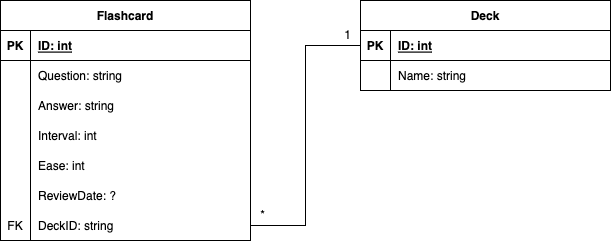
\includegraphics[width=0.4\textwidth]{NerddeckModel.png}
        \caption{Diagram of the Flashcard model based on \ac{uml}}\label{fig:model}
    \end{figure}

\begin{lstlisting}[language=json,firstnumber=1,float=tp, caption={Example of how a flashcard object is saved inside a \ac{json} file}, label=l:flashcardjson]
[{
    "ID": "37268335dd6931045bdcdf926",
    "Question": "What algebraic data types does F# use?",
    "Answer": "Record types and discriminated unions",
    "Repetitions": 1,
    "EasinessFactor": 1.3,
    "NextReview": "2023-12-18T18:17:22.438077+01:00"
}]   
\end{lstlisting}

    \section{Functionality Overview and User Interface}\label{sec:functionalityoverview}
    Figure\ \ref{fig:screenshotcli} displays the prompt inside the \ac{cli} of the F\# implementation. The welcome screen and menu appear identical in the Go implementation. Users can choose from five options when executing the program:        
    \begin{itemize}
        \item \textbf{0. Instructions:} Shows how the program should be used.
        \item \textbf{1. Add flashcard} Add a flashcard and saves it into the \ac{json} file.
        \item \textbf{2. View flashcards:} Just prints all flashcards from the \ac{json} file on the \ac{cli}.
        \item \textbf{3. Start Learning flashcards:} Loads all flashcards from the \ac{json} file. Checks all due flashcards based on the next review. Learn every flashcard and then rate each one from 1 to 4 while 1 is bad and 4 is good. Apply the value as input for the \ac{sm2} algorithm and save the result in the \ac{json} file.
        \item \textbf{4. Exit:} Exit the program.
    \end{itemize}

    \begin{figure}
        \centering
        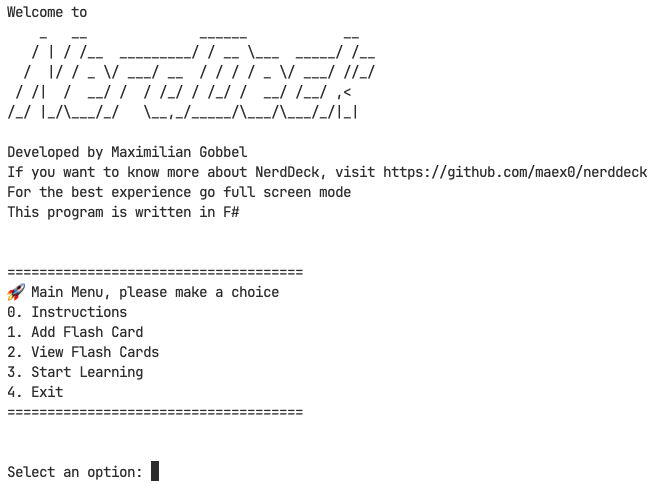
\includegraphics[width=0.76\textwidth]{ScreenshotNerdDeck.png}
        \caption{Screenshot of the \ac{cli} which shows the start of \textit{NerdDeck}}\label{fig:screenshotcli}
    \end{figure}


%========================================================CHAPTER 3========================================================

\chapter{Overview of functional programming}\label{chap:functional-programming}
\begin{shaded}
    \noindent
    \glqq{}As software becomes more and more complex, it is more and more important to structure it well. Well-structured software is easy to write, easy to debug, and provides a collection of modules that can be re-used to reduce future programming costs. Conventional languages place conceptual limits on the way problems can be modularized. Functional languages push those limits back.\grqq{} \cite{Hughes1989}
\end{shaded}

The motivation for using \ac{fp} should be considered. Within the paradigm of \ac{fp}, developers adhere to principles that prioritize the creation of expressive and concise solutions.
    
    \section{Key principles}
    Rooted in mathematical concepts like lambda calculus, \ac{fp} emerges as a methodology characterized by rigor and elegance.
    Key principles integral to \ac{fp} include:
    \begin{itemize}
        \item \textbf{Purity:} Strict avoidance of side effects to ensure deterministic behavior.
        \item \textbf{Higher-order functions:} Utilization of functions as parameters and return values for enhanced modularity.
        \item \textbf{Lazy evaluation:} Selective computation, evaluating values only when necessary for optimization.
        \item \textbf{Algebraic data types:} Incorporation of sum- and product-types, as discussed in more detail in Section\ \ref{sec:algebraic-data-types}.
        \item \textbf{First-class Functions:} A powerful technique, elaborated further in Section\ \ref{sec:first-class-functions}.
    \end{itemize}
    \ac{fp} has a rich history dating back to 1950 with the introduction of the language LISP. Since then, \ac{fp} has evolved across various programming languages, such as like Go and F\#. F\# strictly adheres to a functional-first approach, emphasizing immutability and mathematical principles. In contrast, Go incorporates impure functional elements, showcasing the adaptability of \ac{fp} principles. Chapter\ \ref{chap:introgoandfsharp} provides further insights into this topic. As developers navigate through contrasting algorithms, they reflect on the historical evolution and diversity of \ac{fp} languages. This exploration serves as a testament to the flexibility of programming paradigms and prompts consideration of the nuanced trade-offs between explicit instruction and expressive abstraction within the dynamic context of \ac{fp}. In conclusion, \ac{fp} provides professionals with a robust set of tools, emphasizing immutability, higher-order functions, and mathematical principles.\ \ac{fp} not only addresses current challenges in software development but also promotes a deeper understanding of the complexities involved in designing robust, modular, and expressive code.

    \section{Imperative vs. Declarative}
    Within the programming paradigm spectrum, the imperative and declarative styles represent contrasting approaches to articulating code. This text will demonstrate both approaches using a simple algorithm written in pseudocode for summing up an array of numbers.

    \subsubsection{Imperative Approach}
    Algorithm\ \ref{alg:imperative_sum} exemplifies the imperative paradigm. This paradigm directs the computer through computations using explicit steps. Each line of pseudocode provides instructions to the computer on how to perform the calculation, adhering to traditional imperative paradigms. The sum is explicitly calculated in a \texttt{for loop} from line three to five.

\begin{algorithm}
    \SetKwInOut{Input}{Input}
    \SetKwInOut{Output}{Output}

    \underline{function SumArray} $(a)$\;
    \Input{Integer Array $a$}
    \Output{Sum of elements in $a$}
    
    \BlankLine
    $result \leftarrow 0$
    
    \ForEach{$element$ \textbf{in} $a$}
    {
        $result \leftarrow result + element$
    }
    
    \Return $result$
    
    \caption{Imperative way of summing up an integer array}\label{alg:imperative_sum}
\end{algorithm}

\subsubsection{Declarative Approach}

In contrast, the declarative style, demonstrated by Algorithm\ \ref{alg:declarative_sum}, emphasizes expressing the desired outcome directly rather than detailing step-by-step procedures. This approach is a hallmark of \ac{fp}, leverages the power of functions and abstraction. In chapter\ \ref{chap:introgoandfsharp}, we will encounter a similar concise syntax while using F\#.

\begin{algorithm}
    \SetKwInOut{Input}{Input}
    \SetKwInOut{Output}{Output}

    \underline{function SumArray} $(a)$\;
    \Input{Integer Array $a$}
    \Output{Sum of elements in $a$}
    
    \BlankLine
    \Return $\sum_{\text{element in } a} \text{element}$
    
    \caption{Declarative way of summing up an integer array}
    \label{alg:declarative_sum}
\end{algorithm}


%========================================================CHAPTER 4========================================================

\chapter{Introduction to Go and F\#}\label{chap:introgoandfsharp}
In this chapter, we explore the distinctive features of Go and F\#, offering a brief overview of each language.

    \section{Overview of Go}\label{sec:go-overview}
    Go, commonly known as Golang, is employed to build simple, secure, and scalable systems. It is a statically-typed, compiled programming language designed by Google engineers Robert Griesemer, Rob Pike, and Ken Thompson in 2007. It is used very widely within big companies like Google, Paypal or Netflix. As an open source language, Go is characterized by: 
    \begin{itemize}
        \item \textbf{Concurrent programming:}  Native support through goroutines and channels for scalable and parallelized \ac{app}s.
        \item \textbf{Efficiency:} Statically-typed, compiled that produces standalone binaries. Good for deployment in various environments.
        \item \textbf{Flexibility:} Can be used for Cloud \& Network Services, \ac{cli}s, Web Development and Development Operations \& Site Reliability Engineering.
    \end{itemize}
    \cite{Gowebsite}

    \section{Overview of F\#}\label{sec:fsharp-overview}
    F\# is a functional-first programming language developed by Microsoft Research in 2005.
    Besides C\# and Visual Basic, F\# is another programming language within the .NET ecosystem. On the official website of microsoft it is declared as an open-source language that makes it easy to write succinct, robust, and performant code. Microsoft names itself as a leading contributor. F\# has an active community and support \cite{Fsharpfoundation}.
    While developing, F\# has a very powerful build-in future called \ac{repl}. Besides of that the key features are:
    \begin{itemize}
        \item \textbf{Functional-first:} Immutable by default, First-class functions, Pattern Matching, Algebraic Data Types 
        \item \textbf{Lightweight syntax:} Type inference and automatic generalization
        \item \textbf{Interoperability:} Access .NET Libraries and APIs (e.g. ASP.NET or Entity Framework). 
    \end{itemize}
    \cite{Dotnet}
    \cite{Keyfeaturesfsharp}


%========================================================CHAPTER 5========================================================

\chapter{Comparison of functional concepts}\label{chap:comparison}
To compare the programming languages Go and F\# in the context of \ac{fp}, we will examine two concepts in more detail: Algebraic Data Types and First-class Functions. 

    \section{Algebraic Data Types}\label{sec:algebraic-data-types}

    Algebraic data types are a cornerstone of \ac{fp}, providing a way to model complex data structures. In Go, these types are not directly supported as in languages like F\#, which has native support for discriminated unions and pattern matching. In both Go and F\#, the \texttt{FlashCard} type is used to represent a flashcard, capturing essential information such as the card's ID, question, answer, number of repetitions, ease factor, and the next review date. Despite serving the same purpose, there are syntactic and structural differences between the implementations in Go and F\#.

    \subsection*{F\#}
    F\# provides native support for algebraic data types through record types and discriminated unions. These enable developers to define a set of related values that can be handled concisely and expressively using pattern matching. This feature enhances the readability and maintainability of F\# code, making it a powerful tool for developers who embrace \ac{fp}.

    Listing \ref{l:flashcardfsharp} defines the \texttt{FlashCard} from figure \ref{fig:model} using a record type\footnote{Website: \url{https://learn.microsoft.com/dotnet/fsharp/language-reference/records} (Accessed on 01/08/2024)}. The record contains fields for \texttt{ID}, \texttt{Question}, \texttt{Answer}, \texttt{Repetitions}, \texttt{EFactor}, and \texttt{NextReview}. Records in F\# provide automatically, making them well-suited for representing data with fixed attributes.

    \subsection*{Go}
    In Go, developers commonly use \texttt{struct} types to represent data structures. Although they provide a way to encapsulate related data, they lack the succinct expressiveness of algebraic data types. Go's approach often involves using interfaces and composition to achieve similar outcomes, but this can lead to more verbose code compared to the concise syntax offered by algebraic data types.

    Therefore, the \texttt{FlashCard} type is defined using a \texttt{struct}. This can be seen in listing \ref{l:flashcardgo}. Go structs are mutable, meaning that fields can be updated after creation. Additionally, Go uses explicit types for each field, providing a statically typed approach.

\begin{figure}[ht]
\begin{subfigure}{0.48\textwidth}
\begin{lstlisting}[language=go, firstnumber=1, caption={FlashCard representation in Go}, label=l:flashcardgo]
type FlashCard struct {
    ID          string
    Question    string
    Answer      string
    Repetitions int
    EFactor     float64
    NextReview  time.Time
}
\end{lstlisting}
\end{subfigure}\hfill
\begin{subfigure}{0.48\textwidth}
\begin{lstlisting}[language=FSharp, firstnumber=1, caption={FlashCard representation in F\#}, label=l:flashcardfsharp]
type FlashCard =
    { ID : string
    Question : string
    Answer : string
    Repetitions : int
    EFactor : float
    NextReview : DateTime }
\end{lstlisting}
\end{subfigure}
\caption{Comparison of FlashCard representations in Go and F\#}\label{fig:flashcardcomparison}
\end{figure}

    \section{First-class Functions}\label{sec:first-class-functions}
    Both Go and F\# support first-class functions, treating functions as first-class citizens. In Go, functions can be assigned to variables, passed as arguments, and returned as values. The use of anonymous functions, known as closures, is common in Go, enhancing the \ac{fp} paradigm. Similarly, F\# provides robust support for first-class functions, aligning with its \ac{fp} paradigm. Functions in F\# can be assigned to variables, passed as arguments, and returned as values. The language encourages the use of higher-order functions, enabling powerful abstractions through functions.

    \subsection*{F\#}
    In the F\# example in listing \ref{l:dueforreviewfsharp}, we define a first-class function \texttt{isDueForReview} that checks if a flashcard is due for review based on specific criteria. We then use this function to filter a list of flashcards, to check if a flashcard is due for learning or not. The return value of the function should be a list of due flashcards. As an example in line four, the function is called on the List.filter function. It takes a predicate of type \texttt{T -> bool} and a list as input and returns a list containing only the elements that satisfy the predicate.\footnote{Website: \url{https://fsharp.github.io/fsharp-core-docs/reference/fsharp-collections-listmodule.html\#filter} (Accessed on 01/08/2024)} Moreover, F\# introduces the pipe operator \texttt{|>}, affording developers the convenience of placing the last argument at the forefront. This operator facilitates a more fluid and readable syntax, as exemplified by \texttt{cards |> List.filter isDueForReview}, where the \texttt{isDueForReview} function is seamlessly applied to the \texttt{cards} list through the pipe operator. This expression is equivalent to line four of listing \ref{l:dueforreviewfsharp}. The same functionality should no be implemented in the Go programming language.

\begin{lstlisting}[language=fsharp, firstnumber=1,float=tp, caption={First-class function reresentation in F\#}, label=l:dueforreviewfsharp]
let isDueForReview card =
    card.Repetitions > 0 && card.NextReview <= DateTime.Now
        
let dueFlashCards = List.filter isDueForReview cards
\end{lstlisting}
        
    \subsection*{Go}
    In the Go example in listing \ref{l:flashcardgo}, we define the same first-class function \texttt{isDueForReview} than in F\# that checks if a flashcard is due for review based on specific criteria. The filter function from line six called \texttt{filterDueFlashCards} takes a slice of flashcards (\texttt{cards}) and applies the \texttt{isDueForReview} function to filter out only those flashcards that meet the review criteria. The filtered flashcards are then collected in the \texttt{dueFlashCards} slice and will be returned when all cards are covered.
    
    As an example, line 17 invokes the \texttt{filterDueFlashCards} function with a given set of flashcards (\texttt{cards}) and assigns the resulting list of flashcards due for review to the \texttt{dueFlashCards} variable. This variable encapsulates the outcome of the flashcard filtering process.

\begin{lstlisting}[language=go, firstnumber=1, caption={FlashCard representation in F\#}, label=l:dueforreviewgo]
func isDueForReview(card FlashCard) bool {
    return card.Repetitions > 0 
    && card.NextReview.Before(time.Now())
}

func filterDueFlashCards(cards []FlashCard) []FlashCard {
    var dueFlashCards []FlashCard
    for _, card := range cards {
        if isDueForReview(card) {
            dueFlashCards = append(dueFlashCards, card)
        }
    }
    return dueFlashCards
}


dueFlashCards := filterDueFlashCards(cards)
\end{lstlisting}
            

    \section{Key Takeaway}\label{sec:keytakeaway}
    While Go's \texttt{struct} types are mutable by default, F\#'s \texttt{record} types are immutable by default. Immutability simplifies reasoning about state and enables certain optimizations. It is worth noting that every field in Go must have an explicitly defined type, whereas in F\#, they are inferred based on their usage. Neither language supports inheritance. Both languages support first-class functions, making them suitable choices for developers with different preferences in balancing imperative and \ac{fp} styles. The difference between the two languages lies in their syntax and expressiveness. This can be seen in each of the four examples in listing \ref{l:flashcardgo}, \ref{l:flashcardfsharp}, \ref{l:dueforreviewfsharp} and \ref{l:dueforreviewgo}. It is worth noting that neither language is completely pure. While Go allows for mutation, even F\#, which is primarily a functional language, permits its use.


%========================================================CHAPTER 5========================================================

\chapter{Conclusion}\label{chap:conclusion}
This paper analyzes and compares key concepts, such as algebraic data types and first-class functions, within the context of \ac{fp} paradigms in Go and F\#. The \textit{NerdDeck} flashcard \ac{app} served as a practical example to illustrate the application of \ac{fp} principles in both languages. The comparison revealed distinctions in their approaches, showcasing F\#'s native support for \ac{fp} and Go's adaptation within its multi-paradigm framework.

    \section{Challenges}\label{sec:challenges}
    The foundation of a good comparison in the context of this paper is to write code as pure as possible to fulfill the paradigm of \ac{fp}. However, challenges arose due to the inherent impurity in both Go and F\#. While F\# aligns more closely with \ac{fp} principles, Go's multi-paradigm nature required creative workarounds to achieve a functional style. This emphasizes the importance of navigating the balancing between functional and imperative programming in each language. The challenges also highlight the need for a nuanced approach when selecting a language for projects where \ac{fp} principles and their advantages are a priority.        

    \section{Outlook}\label{sec:outlook}
    Looking ahead, there is potential for further exploration into writing more pure functional code within the \textit{NerdDeck} or similar projects. To achieve this, a pure programming language such as Haskell\footnote{Website: \url{https://www.haskell.org} (Accessed on 12/20/2023)} could be considered. This would involve delving deeper into \ac{fp} concepts and finding innovative solutions within the constraints of a specific language. Additionally, as programming languages and paradigms continue to evolve, ongoing advancements may present new opportunities and challenges for \ac{fp} practitioners. The insights gained from this comparative analysis contribute to a broader understanding of \ac{fp} in diverse language ecosystems and provide a foundation for future exploration and research.
